\documentclass[12pt]{article}
\setlength{\oddsidemargin}{0in}
\setlength{\evensidemargin}{0in}
\setlength{\textwidth}{6.5in}
\setlength{\parindent}{0in}
\setlength{\parskip}{\baselineskip}

\usepackage{amsmath,amsfonts,amssymb,bm,graphics,pgfplots,framed,dsfont}
\usepackage[scale=0.75,top=1cm,bottom=3cm]{geometry}

\begin{document}

\textbf{Minh Anh Nguyen }\\
\textbf{Calculus 1 Assignment-10}\\
\textbf{Section: 04}\\
\textbf{TA's name: Arthur Huey}

\hrulefill

\begin{enumerate}
\setcounter{enumi}{6}
    \item A table of values of an increasing function $f$ is shown. Use the table to find the lower and upper bound estimates of $\int_{10}^{30} f(x)dx$
    \begin{center}
        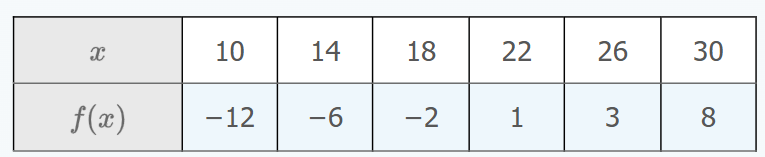
\includegraphics[scale=0.5]{img/img-0.png}
    \end{center}
    \[Lower = 4\times(-12 + -6 + -2 + 1 + 3) = -64\]
    \[Upper = 4\times(-6 + -2 + 1 + 3 + 8) = 16\]
\setcounter{enumi}{10}
    \item Use the Midpoint Rule with the given value of $n$ to approximate the integral. Round the answer to four decimal places.
    \[\int_{0}^{8} \sin \sqrt{x} \text{ } dx, n = 4\]
    \[\Delta x = \frac{8-0}{4} = 2\]
    \[\int_{0}^{8} \sin \sqrt{x} \approx 2 \times (f(\frac{2+0}{2}) + f(\frac{4+2}{2}) + f(\frac{6+4}{2}) + f(\frac{8+6}{2})) \approx 6.1820\]
\setcounter{enumi}{18}
    \item Express the limit as a definite integral on the given interval.
    \[\lim_{n \to \infty} \Sigma_{i=1}^{n} \frac{\sin x_i}{1 + x_i}\Delta x, [0,\pi]\]
    \[\lim_{n \to \infty} \Sigma_{i=1}^{n} \frac{\sin x_i}{1 + x_i}\Delta x = \int_{0}^{\pi} \frac{sin x}{1 + x} dx\]
\setcounter{enumi}{22} 
    \item Show that the definite integral is equal to $\lim_{n \to \infty} R_n$ and then evaluate the limit.
    \[\int_{0}^{4}(x-x^2)dx, R_n = \frac{4}{n} \Sigma_{i = 1}^{n}[\frac{4i}{n} - \frac{16i^2}{n^2}]\]
    \[\Delta x = \frac{4-0}{n} = \frac{4}{n}\]
    \[x_i = \frac{4i}{n}\]
    According to Riemann Sum:
    \[\int_{0}^{4}(x-x^2)dx = R_n = \frac{4}{n} \Sigma_{i = 1}^{n}[\frac{4i}{n} - \frac{16i^2}{n}]\]
    \[R_n = \frac{4}{n} \Sigma_{i = 1}^{n}[\frac{4i}{n} - \frac{16i^2}{n^2}] = \frac{4}{n} \Sigma_{i = 1}^{n}\frac{4i}{n} - \frac{4}{n} \Sigma_{i = 1}^{n} \frac{16i^2}{n^2}\]
    \[ = \frac{16}{n^2} \Sigma_{i = 1}^{n}i - \frac{64}{n^3} \Sigma_{i = 1}^{n} i^2 = \frac{16}{n^2} \frac{n(n+1)}{2} - \frac{64}{n^3} \frac{n(n+1)(2n+1)}{6}\]
    \[ = \frac{16(n+1)}{2n} - \frac{64(n+1)(2n+1)}{6n^2}\]
    \[\lim_{n \to \infty} R_n = \lim_{n \to \infty} \frac{16(n+1)}{2n} - \frac{64(n+1)(2n+1)}{6n^2} = \lim_{n \to \infty} \frac{16(n+1)}{2n} - \lim_{n \to \infty} \frac{64(n+1)(2n+1)}{6n^2}\]
    \[ = \lim_{n \to \infty} \frac{16(1+1/n)}{2} - \lim_{n \to \infty} \frac{64(1+1/n)(2+1/n)}{6} = 8 - \frac{128}{6} = - \frac{40}{3}\]
\setcounter{enumi}{30}
    \item Use the form of the definition of the integral given in Theorem 4 to evaluate the integral.
    \[\int_{1}^{5} (3x^2+7x)dx\]
    \[\Delta x = \frac{5-1}{n} = \frac{4}{n}\]
    \[x_i = 1 + \frac{4i}{n}\]
    \[\int_{1}^{5} (3x^2+7x)dx = \lim_{n \to \infty} \Sigma_{i=1}^{n} (3(1+\frac{4i}{n})^2+7(1+\frac{4i}{n})) \frac{4}{n} = \lim_{n \to \infty} \Sigma_{i=1}^{n} (3 + \frac{24i}{n} + \frac{48i^2}{n^2}+7+\frac{28i}{n}) \frac{4}{n} \]
    \[ = \lim_{n \to \infty} \Sigma_{i=1}^{n} (10 + \frac{52i}{n} + \frac{48i^2}{n^2}) \frac{4}{n}  = \lim_{n \to \infty} (\Sigma_{i=1}^{n} 10 + \frac{52}{n} \Sigma_{i=1}^{n} i + \frac{48}{n^2}\Sigma_{i=1}^{n}i^2 ) \frac{4}{n}  \]
    \[ = \lim_{n \to \infty} (10n + \frac{52}{n} \frac{n(n+1)}{2} + \frac{48}{n^2} \frac{n(n+1)(2n+1)}{6})\frac{4}{n} \]
    \[ = \lim_{n \to \infty} (40 + \frac{208}{n^2} \frac{n(n+1)}{2} + \frac{192}{n^3} \frac{n(n+1)(2n+1)}{6})\]
    \[ = \lim_{n \to \infty} (40 + 208 \frac{(1+1/n)}{2} + 192 \frac{(1+1/n)(2+1/n)}{6})\]
    \[ = 40 + 104 + 64 = 208\]
\setcounter{enumi}{40}
    \item Evaluate the integral by interpreting it in terms of areas.
    \[\int_{-2}^{5} (10 - 5x) dx\]
    Because x = 2 is where the function change from positive to negative.
    \[\int_{-2}^{5} (10 - 5x) dx = \int_{-2}^{2} (10 - 5x) dx + \int_{2}^{5} (10 - 5x) dx = \frac{1}{2}(4 \times 20 + 3 \times (-15)) = 40 - 45/2 = 17.5\]
\setcounter{enumi}{51}
    \item Given that $\int_{0}^{\pi} \sin^4 x dx = \frac{3}{8}\pi$, what is $\int_{\pi}^{0} \sin^4 \theta d\theta$.
    \[\int_{\pi}^{0} \sin^4 \theta d\theta = \int_{\pi}^{0} \sin^4 x dx = - \int_{0}^{\pi} \sin^4 x dx = - \frac{3}{8}\pi\]
\setcounter{enumi}{64}
    \item Use the properties of integrals to verify the inequality without evaluating the integrals.
    \[\int_{0}^{4}(x^2-4x+4) dx \geq 0\]
    Because $f(x) = x^2 -4x + 4 = (x-2)^2 \geq 0$ with all $0 \leq x \leq 4$. \\ 
    Hence, $\int_{0}^{4}(x^2-4x+4) dx \geq 0$.  
\end{enumerate}
\end{document}